% !TeX document-id = {3ffda977-020f-403a-a748-6559a1e64ed1}
% !TeX TXS-program:compile = txs:///pdflatex/[--shell-escape]
% % !TEX TS-program = xelatex
% !TEX encoding = UTF-8 Unicode


% Spring 2020 - Summer 2020 - Fall 2020 - SPring 2021
% Tristan Hill, May 07, 2020 - June 12, 2020 - July 08, 2020 - Novemeber 02, 2020 - March 28, 2021
% Module Name: - Electrical Signals
% Topic 2 - Signal Analysis

\documentclass[fleqn]{beamer} % for presentation (has nav buttons at bottom)

\usepackage{/home/thill/Documents/lectures/measurements_lectures/measurements_lectures}


\author{ME3023 - Measurements in Mechanical Systems} % original formatting from Mike Renfro, September 21, 2004

%\newcommand{\MNUM}{9\hspace{2mm}} % Module number - The module number should be phased out...
\newcommand{\TNUM}{2\hspace{2mm}} % Topic number - Topic numbers are going to stay
\newcommand{\moduletitle}{Electrical Signals}
\newcommand{\topictitle}{Signal Analysis} 

\newcommand{\sectiontitleI}{Signal Mean Value}
\newcommand{\sectiontitleII}{Power Dissipation}
\newcommand{\sectiontitleIII}{Signal Root Mean Square (RMS) Value}
\newcommand{\sectiontitleIV}{Discrete-Time or Digital Signals}

\newcommand{\btVFill}{\vskip0pt plus 1filll}


% custom box
\newsavebox{\mybox}

\title{Lecture Module - \moduletitle}

\date{Mechanical Engineering\vspc Tennessee Technological University}

\begin{document}

\lstset{language=MATLAB,basicstyle=\ttfamily\small,showstringspaces=false}

\frame{\titlepage \center\begin{framed}\Large \textbf{Topic \TNUM - \topictitle}\end{framed} \vspace{5mm}}

% Section 0: Outline
\frame{
\large \textbf{Topic \TNUM - \topictitle} \vspace{3mm}\\

\begin{itemize}

	\item \sectiontitleI    \vspc % Section I
	\item \sectiontitleII 	\vspc % Section II
	\item \sectiontitleIII 	\vspc %Section III
	\item \sectiontitleIV 	\vspc %Section IV
%	\item \sectiontitleV 	\vspc %Section IV

\end{itemize}

}

% Section I:
\section{\sectiontitleI}

	% Section I - Frame I:
	\begin{frame}[label=sectionI] \small
		\frametitle{\sectiontitleI}

		\begin{multicols}{2}
		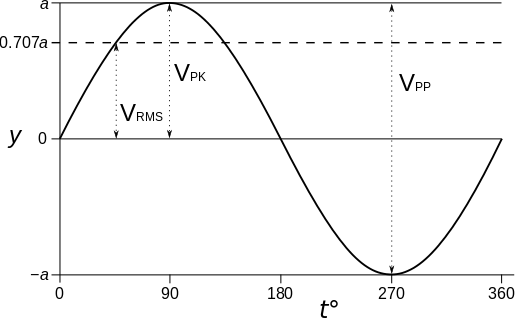
\includegraphics[scale=.30]{amplitude_frequency.png} 
		
 Mean Value \[\bar{y}\equiv \frac{\int\limits_{t_1}^{t_2} y(t)dt}{\int\limits_{t_1}^{t_2} dt} \]
		\end{multicols}
		\btVFill
		\tiny{Text: Theory and Design for Mechanical Measurements}
	\end{frame}

\section{\sectiontitleII}	
	% Section II - Frame I
	\begin{frame}[label=sectionII] \small
		\frametitle{\sectiontitleII}
Dissipation - Time Rate of Energy Dissipation    \[ P=I^2R \]  
	
	Total Electrical Energy \hspace{5mm} \[ E =\int\limits_{t_1}^{t_2}P dt=\int\limits_{t_1}^{t_2}[I(t)]^2R dt \]
		
		
	\end{frame}

	
\section{\sectiontitleIII}	

% Section III - Frame I
\begin{frame}[label=sectionIII] \small
\frametitle{\sectiontitleIII}
\bigskip

	\begin{itemize}
	\item For a cyclically alternating electric current, RMS is equal to the value of the direct current that would produce the same average power dissipation in a resistive load.
	\item In Estimation theory, the root mean square error of an estimator is a measure of the imperfection of the fit of the estimator to the data.  
	\item The RMS value of a signal having a zero mean is a statistical measure of the magnitude of the fluctuations in the signal.
	\end{itemize}

\btVFill
\tiny{Text: \href{https://en.wikipedia.org/wiki/Root_mean_square\#In_electrical_engineering}{wikipedia}}		

\end{frame}

% Section III - Frame II
\begin{frame}[label=sectionIII] \small
\frametitle{\sectiontitleIII}
\bigskip


\btVFill
\tiny{Table 2.1 : Theory and Design for Mechanical Measurements}	
\end{frame}

\section{\sectiontitleIV}	

% Section IV - Frame I
\begin{frame}[label=sectionIV] \small
\frametitle{\sectiontitleIV}
\bigskip

\[\bar{y}=\frac{1}{N}\sum\limits_{i=0}^{N-1} y_i\] \vspace{10mm}\\	
\[y_{RMS}=\sqrt{\frac{1}{N}\sum\limits_{i=0}^{N-1} y_i^2}\] \vspace{10mm}\\	

\btVFill
\tiny{Text: Theory and Design for Mechanical Measurements}	
\end{frame}

% Section IV - Frame II
\begin{frame}[label=sectionIV] \small
\frametitle{\sectiontitleIV}
\bigskip



\btVFill
\tiny{Table 2.1 : Theory and Design for Mechanical Measurements}	
\end{frame}

\end{document}
